\documentclass[a4paper, 12pt]{article}
\usepackage{comment} 
\usepackage{fullpage}
\usepackage[hidelinks]{hyperref}
\usepackage{amsmath}
\usepackage{environ}
\usepackage{algorithm}
\usepackage{algpseudocode}
\usepackage{graphicx}
\usepackage{tabto,enumitem}


\begin{document}
\noindent
\large\textbf{SOEN 6011} \hfill \textbf{Aniket Tailor}\\
\large\textbf{Software Engineering Processes} \hfill \textbf{40195068} \\
Function 8 : Standard Deviation $\sigma$ \hfill Date: 5 August 2022\\
\normalsize Problem 3 \\
\section*{Algorithms for Standard Deviation}
\textbf{1. Pseudo code of Traditional (Iterative) approach}\\

\begin{algorithm}
\caption{Traditional Algorithm}

\begin{algorithmic}[1]

\Procedure{StandardDeviation}{\;}
    \State $Sum \leftarrow 0$
    \State $Mean \leftarrow 0$
    \State $Var \leftarrow 0$
    \State $SD \leftarrow 0$
    \State $Number \leftarrow 0$
    \State $Size \leftarrow \;Array.count()$
    \State $Sum \leftarrow \;Sum+Sum$
    \For{$i \leftarrow 0,size$}
    \State $Sum+=Array$
    \EndFor
    \State $SD=squareRoot(SD/Size)$
    \State \textbf{Return} SD
    \EndProcedure
\Statex
\end{algorithmic}
\end{algorithm}

\section*{Which one to choose, Traditional or N-Pass?}
\begin{itemize}[noitemsep]
        \item Standard deviation can be calculated more quickly and with considerably more efficiency using the n-pass technique, which can accept more data inputs in the form of files. Other than that, the problem is that because it employs recursion rather than iteration, the memory stack would fill up quickly.
        \item The standard deviation can be calculated using the traditional approach, but it can take some time if the input data is huge and the frequency of the numbers is high. In addition, it is more prone to errors. As a result, the Multi pass or n-pass algorithm is more faster and more effective than the Traditional approach for standard deviation.

    \end{itemize}

\newpage
\section*{Algorithms for Standard Deviation}
\textbf{2. Pseudo code of N-Pass approach}\\
\begin{algorithm}
\caption{N-Pass Algorithm}
\begin{algorithmic}[1]

\Procedure{StandardDeviation}{\;}
    \State $Size \leftarrow \;Array.count()$
    \For{$i \leftarrow 0,size$}
    \State $Sum+=Array$
    \EndFor
    \State $Mean \leftarrow Sum/Size$
    \For{$i \leftarrow 0,size$}
    \State $SD=SD+power((Array[i]-Mean),2)$
    \EndFor
    \State $Variance=SD/Size$
    \State $SD=SquareRoot(Variance)$    
    \State \textbf{Return} SD
    \EndProcedure
\Statex
\Procedure{Power}{x,y}
    \For{$i \leftarrow 1,y$}
    \State $Result=Result*x$
    \EndFor
    \State \textbf{Return} Result
    \EndProcedure
\Statex
\Procedure{SquareRoot}{x}
    \State $temp$
    \State $sqrt \leftarrow \frac{x}{2}$
    \State $temp \leftarrow sqrt$
    \State $sqrt \leftarrow \frac{temp +\frac{x}{temp}}{2} $
    \While{$temp - sqrt \neq 0$}
    \State $temp \leftarrow sqrt$
    \State $sqrt \leftarrow \frac{temp +\frac{x}{temp}}{2} $
    \EndWhile
    \State \textbf{Return} $temp$
    \EndProcedure
\Statex
\end{algorithmic}
\end{algorithm}
\newpage
\section*{Mind Map}
The below given mind map shows the flow of the pseudo code for finding Standard Deviation. The algorithm will start from Main() method by taking input of data values. It will then call the CalculateSum() procedure to calculate sum of the data elements. With mean and array size in hand, CalculateVariance() method will be called. Internally this method calls Power() function to compute power and atlast SquareRoot() is used to find Standard Deviation.\\  
\begin{figure}[h]
    \centering
    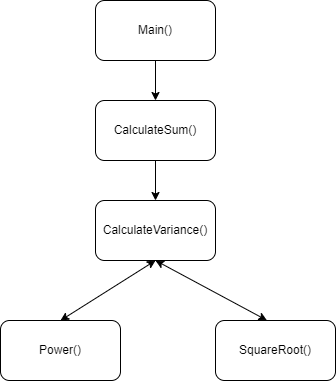
\includegraphics{Images/mindmap.png}
    \caption{Mind Map}
    \label{fig:Mind Map Image}
\end{figure}
\newpage
\section*{Pros of Traditional Algorithm}
\begin{itemize}
        \item This method does not uses the stack so it's faster.
        \item Traditional algorithm consumes less memory.
        \item The code is easy to understand and debug.
    \end{itemize}
\section*{Cons of Traditional Algorithm}
\begin{itemize}
        \item The iterative alternative is to repeatedly dynamically allocate or resize memory blocks. On many platforms automatic allocation is much faster, to the point that its speed bonus outweighs the speed penalty and storage cost of recursive calls.
        \item It makes the code longer.
        \item Sometimes execution and calculation time becomes higher.
    \end{itemize}
\section*{Pros of N-Pass Algorithm}
\begin{itemize}
        \item It is faster and much more efficient to use because it makes use of memory upto the mark. 
        \item Can take large set of data to find standard deviation.
        \item It makes the code smaller.

    \end{itemize}
\section*{Cons of N-Pass Algorithm}
\begin{itemize}
        \item The inbuilt garbage collector begins to operate when the memory stack becomes mostly full, deleting the unused memory that has filled the stack.

    \end{itemize}
    
\newpage
\begin{thebibliography}{15}

\addcontentsline{toc}{chapter}{Bibliography}
\bibitem{1}
\href{https://benpfaff.org/writings/clc/recursion-vs-iteration.html#:~:text=The\%20iterative\%20alternative\%20is\%20to,storage\%20cost\%20of\%20recursive\%20calls.}{https://benpfaff.org/writings/clc/recursion-vs-iteration.html}

\bibitem{2}
\href{https://www.tutorialspoint.com/what-are-the-differences-between-recursion-and-iteration-in-java}{https://www.tutorialspoint.com/what-are-the-differences-between-recursion-and-iteration-in-java}

\bibitem{3}
\href{https://influentialpoints.com/Training/variance_and_standard_deviation-principles-properties-assumptions}{https://influentialpoints.com/Training/variance\_and\_standard\_deviation-principles-properties-assumptions}

\end{thebibliography}
\end{document}